% !TEX program=lualatex
\RequirePackage{luatex85}
\documentclass[tikz,border=10,10pt]{standalone}

\usepackage{amsmath}
\usepackage{amssymb}
\usepackage{mathtools}
\usepackage{unicode-math}
\usepackage{fontspec}
\usepackage{microtype} % Slightly tweak font spacing for aesthetics
\usepackage{xcolor}

\usepackage{tikz}
\usetikzlibrary{shapes,arrows,positioning}
\tikzset{
  font={\fontsize{9pt}{11}\selectfont}
}

\setmainfont{TeX Gyre Heros}
\setmathfont{Latin Modern Math}

\definecolor{colorR}{RGB}{228,26,28}    % RED
\definecolor{colorB}{RGB}{55,126,184}   % BLUE
\definecolor{colorG}{RGB}{77,175,74}    % GREEN
\definecolor{colorP}{RGB}{152,78,163}   % PURPLE
\definecolor{colorO}{RGB}{255,127,0}    % ORANGE
\definecolor{colorY}{RGB}{255,255,51}   % YELLOW
\definecolor{colorBn}{RGB}{166,86,40}   % BROWN
\definecolor{colorPk}{RGB}{247,129,191} % PINK
\definecolor{colorGy}{RGB}{153,153,153} % GRAY

\tikzstyle{line}=[draw, -stealth', very thick]
\tikzstyle{block}=[circle,fill=colorB!50,on grid]
\tikzstyle{lab}=[]
\tikzstyle{w}=[lab,midway]
\tikzstyle{e}=[lab,midway,auto=false,fill=colorP!50,font=\scriptsize]
\tikzstyle{p}=[lab,midway,auto=false,fill=colorO!50,font=\scriptsize]

\begin{document}
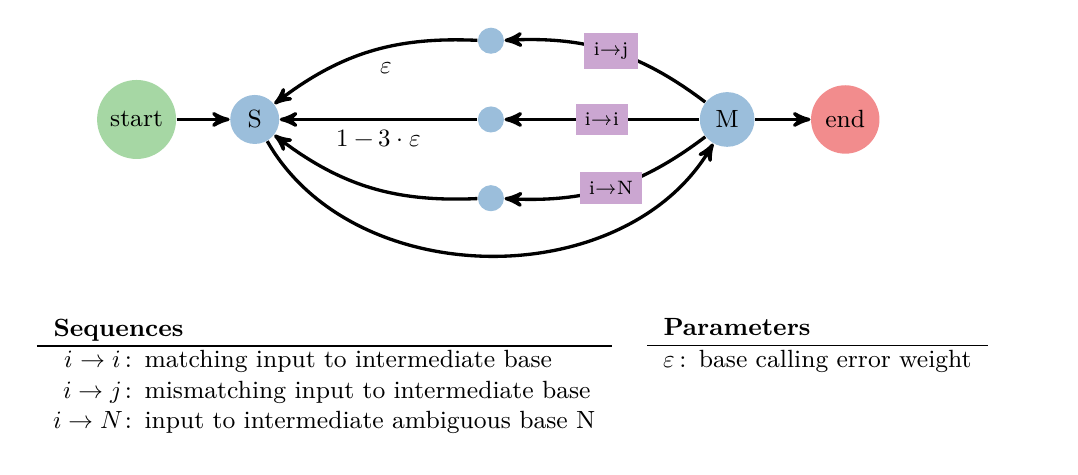
\begin{tikzpicture}[node distance=25mm, auto,
	dottedline/.style = {ultra thick, loosely dotted,shorten >=1mm, shorten <=1mm}]
%\node (titlea) {\textbf{Base Calling Error FST}};

\node[block,fill=colorG!50] (start_sub) {start};
\node[block,right=15mm of start_sub] (S_sub) {S};
\node[block,above right=10mm and 30mm of S_sub] (ij_sub) {};
\node[block,right=30mm of S_sub] (ii_sub) {};
\node[block,below right=10mm and 30mm of S_sub] (in_sub) {};
\node[block,right=60mm of S_sub] (M_sub) {M};
\node[block,fill=colorR!50,right=15mm of M_sub] (end_sub) {end};

\draw[line] (start_sub) -- (S_sub);
\draw[line] (M_sub) -- (end_sub);

\draw[line] (M_sub) to[bend right=20] node[e] {i\textrightarrow{}j} (ij_sub);
\draw[line] (ij_sub) to[bend right=20] node[w] {$\varepsilon$} (S_sub);
\draw[line] (M_sub) to node[e] {i\textrightarrow{}i} (ii_sub);
\draw[line] (ii_sub) to node[w] {$1 - 3 \cdot \varepsilon$} (S_sub);
\draw[line] (M_sub) to[bend right=-20] node[e] {i\textrightarrow{}N} (in_sub);
\draw[line] (in_sub) to[bend right=-20] (S_sub);

\draw[line] (S_sub) to[bend left=-60] (M_sub);

%%% Legend

\node[below right=2cm and -1.75cm of start_sub,text width=50mm,anchor=north west] (sequences) {
\begin{tabular}{r@{\,: }l}
\multicolumn{2}{l}{\textbf{Sequences}}\\
    \hline
	$i \rightarrow i$ & matching input to intermediate base\\
	$i \rightarrow j$ & mismatching input to intermediate base\\
	$i \rightarrow N$ & input to intermediate ambiguous base N\\
\end{tabular}
};

\node[above right=-1.03cm and 25mm of sequences,text width=50mm] {
\begin{tabular}{r@{\,: }l}
\multicolumn{2}{l}{\textbf{Parameters}}\\
\hline
	$\varepsilon$ & base calling error weight\\
\end{tabular}
};

\end{tikzpicture}
\end{document}
